\documentclass{article}
\usepackage{graphicx}
\usepackage{float}
\begin{document}

Name: Thao, Nguyen Van.   Id: ic87adyh
\section*{\textbf{I. Problem 1.2 (Disjunctive Random Variables)}}

$P(A \lor B \lor C) = P(A) + P(B) + P(C) - P(A \land B) - P(A \land C) - P(B \land C) + P(A \land B \land C)$

To find the probability of A or B or C, we start by adding the probabilities of A, B, and C. However, we have counted the overlapping regions twice, so we need to subtract the probabilities of the overlaps (A and B, A and C, and B and C). Then, we need to add back the probability of the region where all three circles overlap (A and B and C), since it was subtracted twice.  Hence,   the entire diagram (see Figure~\ref{fig:ven_diagram}) represents the union of all three events,  $P(A \lor B \lor C)$   .

\begin{figure}[H]
  \centering
  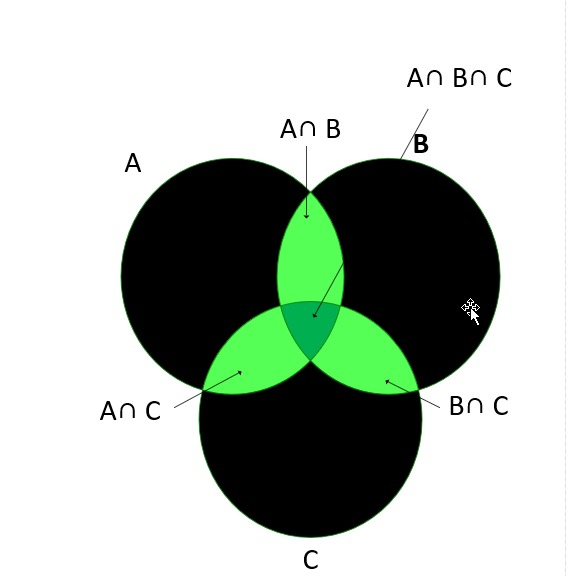
\includegraphics[width=0.5\textwidth]{ven_diagram.jpeg}
  \caption{Venn diagram}
  \label{fig:ven_diagram}
\end{figure}
\end{document}